\subsection{Natural Joins}

The \emph{natural~join} \( R \bowtie S \) of two relations \( R \) and \( S \) is the set of all combinations of the tuples of \( R \) and \( S \) whose common attributes are equal.

\begin{figure}[htp]
  \centering
  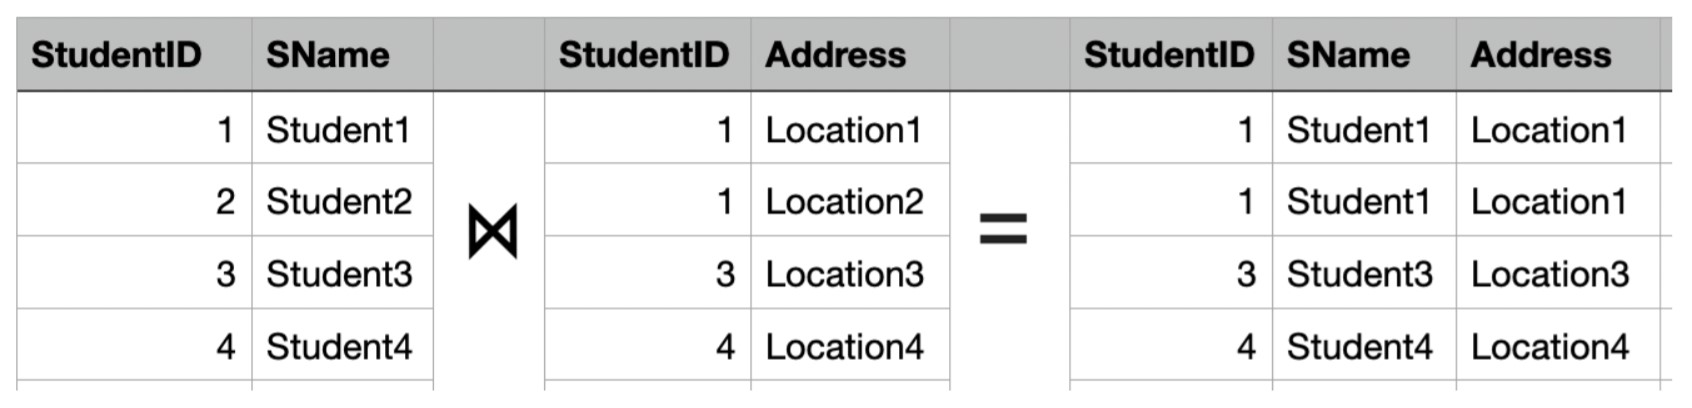
\includegraphics[width=0.8\textwidth]{unit-8/figures/natural-join.jpg}
  \caption*{The natural join of two relations.}
\end{figure}


\subsection{Decomposition of a Relation}

The decomposition of a relation \( R \), whose attributes are the set \( \itol{A} = \left\{ a_1, a_2, \ldots, a_m \right\} \), results in the creation of two new relations \( R_1 \) and \( R_2 \), whose attributes are the sets \( \itol{B} = \left\{ b_1, b_2, \ldots, b_n \right\} \) and \( \itol{C} = \left\{ c_1, c_2, \ldots, c_p \right\} \), respectively, such that \( R_1 \) and \( R_2 \) together contain all the attributes of \( R \), and the natural~join of \( R_1 \) and \( R_2 \) gives \( R \) exactly --- no more, no less.

Thus, all decomposed relations exhibit the following properties.
\begin{equation*}
  \itol{B} \cup \itol{C} = \itol{A}
\end{equation*}
\begin{equation*}
  R_1 \bowtie R_2 = R
\end{equation*}

\subsection{Identification of Boyce-Codd Normal Form (BCNF)}

A relation \( R \) is in \emph{Boyce-Codd Normal Form (BCNF)} if, and only if, for each of its functional dependencies \( \itol{A} \rightarrow \itol{B} \), \( \itol{A} \) is a key.

A functional dependency that causes a relation not to be in BCNF is called a \emph{BCNF~violation}.

\subsection{BCNF Decomposition Algorithm}

In order to decompose the relation \( R \),
\begin{enumerate}
  \item compute the keys of \( R \), then
  \item until all relations are in BCNF,
  \begin{enumerate}
    \item pick any of the problem relations \( R' \) with at least one functional dependency \( \itol{A} \rightarrow \itol{B} \) that violates BCNF (where \( \itol{A} \) is not a key),
    \item decompose it into two relations \( R_1\!\left( \itol{A}, \itol{B} \right) \) and \( R_2\!\left( \itol{A}, \text{rest} \right) \) --- discarding the original relation \( R' \), then
    \item compute the functional dependencies of \( R'_1 \) and \( R'_2 \), and
    \item compute the keys of \( R'_1 \) and \( R'_2 \).
  \end{enumerate}
  \item Finally, the remaining relations \( R' \) are the decomposition of the original relation \( R \).
\end{enumerate}

\begin{figure}[htp]
  \centering
  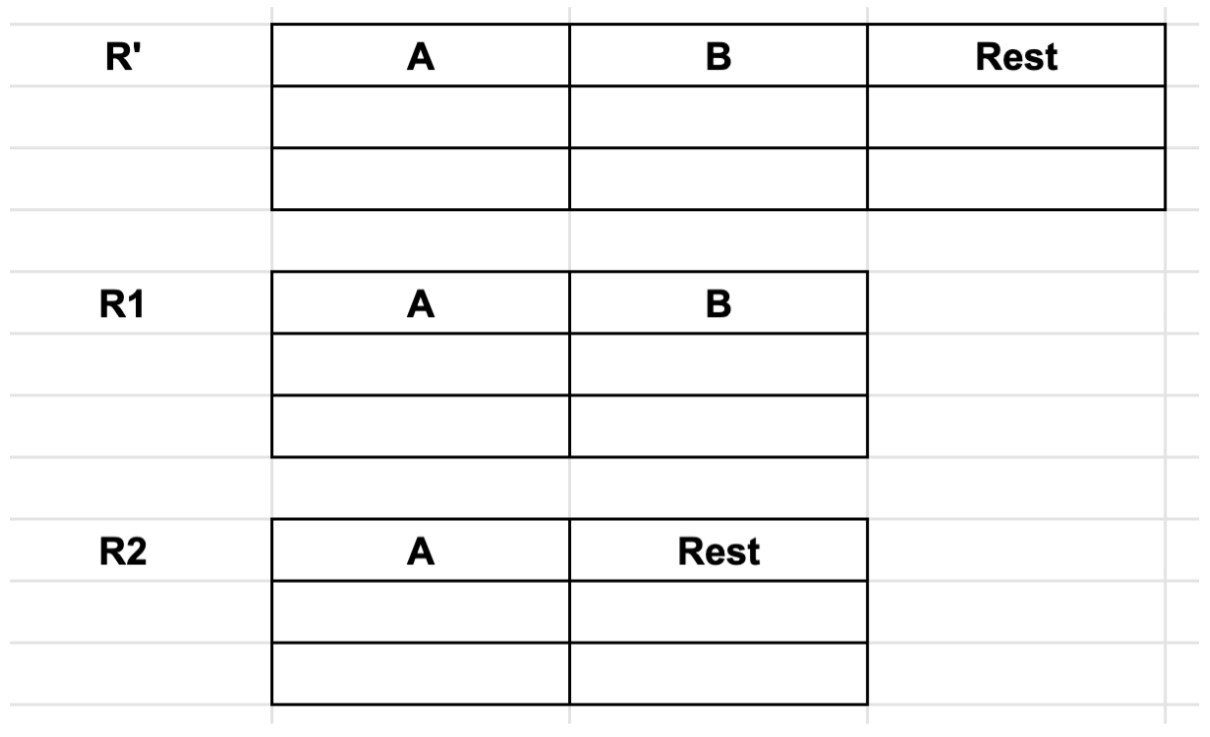
\includegraphics[width=0.6\textwidth]{unit-8/figures/decomposition.jpg}
  \caption*{Decomposition of a relation \( R'\!\left( \itol{A}, \itol{B}, \text{rest} \right) \) into \( R'_1\!\left( \itol{A}, \itol{B} \right) \) and \( R'_2\!\left( \itol{A}, \text{rest} \right) \).}
\end{figure}

The natural join of the decomposed relations \( R' \) is the original relation \( R \), and the union of the attributes of all \( R' \) is the set of attributes of \( R \).

BCNF provides the termination condition for decomposition.
A relation should be decomposed only if at least one of its functional dependencies is a BCNF~violation, and decomposition must continue until all relations are in BCNF, i.e. until there exists no relation with a functional dependency whose independent attributes are not a key.

\subsection{Anomalies}
The term "anomaly" is used to describe these situations (means strangeness).
Anomalies make queries give wrong results, often in a way that we can’t even tell that they are wrong.
Even when we detect that they are wrong, it may be quite difficult to write correct queries to avoid the problem!

\subsubsection{Typology of anomalies} 
\begin{enumerate}
  \item Update anomaly:
When information is updated, we would need to update also the attributes dependent on the updated information.
  \item Insertion anomaly:
When a new record is inserted, we would need to check that the dependent attributes are consistent with the existing ones. (A lot of work!)
  \item Aggregation anomaly:
Aggregation operators (count, sum, average etc.) may give wrong results because of duplication of data.
  \item Deletion anomaly:
If we delete all the records containing a particular value, all its dependent attributes will also be lost.
\end{enumerate}

\subsubsection{Deletion anomaly example}
Consider the schema:
Staff(sid, last name, first name, office, phone)
Suppose we don't store office and phone information anywhere else.
We have an unwanted dependency: office → phone
Deletion anomaly: Suppose everybody in an office leaves and we delete their records. Now we have lost the information about the phone number of that office.


\textbf{Aggregation anomaly example} \\
Consider the schema:
Lecturing(sid, cid, year, numbers)
“numbers” is the number of students in the course during that year.
Aggregation query: Find the average number of students in the courses taught in year 2021.
Since some courses have multiple lecturers (sid's) and others don’t, the average we get from the straightforward query would be wrong. 
See paragraph 90 for a discussion of this example.

A candidate key in a table is a collection of attributes that is unique across all the records.
Primary keys are candidate keys, but there can also be other candidate keys (see paragraph 53 for an example).
A candidate key uniquely determines every other attribute in the record.
$K_1,K_2,....K_n \rightarrow X$
   These functional dependencies are natural and “good”. 
Any other functional dependency, which is not on a candidate key, is considered an “unwanted” functional dependency. It needs to be eliminated.


\textbf{Boyce-Codd normal form:}
\begin{itemize}
  \item A collection of table schemas is said to be in Boyce-Codd normal form (BCNF), if all functional dependencies in all the tables are only on the candidate keys of the tables.\\
This is a bit imprecise. More precise definition to come later.
  \item The term "on the candidate key" can be made precise: \\
  \textcolor{red}{The LHS of every functional dependency must be a superset of a candidate key.}
  \item This is also called the "Fourth normal form" (but we are not covering this typology of normal forms.)
  \item The way to get tables into BCNF is to decompose table that have “unwanted” functional dependencies, which are not on the candidate keys.
\end{itemize}

Decomposition (normalisation) method
Suppose you have an unwanted functional dependency $U \rightarrow X$
We first find all the attributes that are functionally dependent on U the left hand side of the functional dependency
(using the closure algorithm of paragraph 82).
Suppose W is the collection of attributes functionally dependent on U.
Let the remaining attributes (other than U and W) be V.
Then we have the picture of the next slide.

If we join the two decomposed tables $S_1$ and $S_2$, we will get back exactly the original table.
This is a theorem! It is called "losslessness". Paragraph 87.
It is clear that every record of the original table will be regained when we join $S_1$ and $S_2$. \\
But the question remains whether we will get any new records, which were not present in the original table S.\\
Suppose we get a new record $x_V x_U x_W$. That means $x_V x_U y_W$, for some $y_W$, must have been present in $S$.
This would have given records $x_V x_U$ in $S_1$ and $x_U y_W$ in $S_2$.
This is not possible unless $x_W=y_W$ because $U$ functionally determines every attribute in $W$.
So new records cannot be present in the joined table.

Design theorists worry about three properties of decompositions: \\
Losslessness. 
\begin{itemize}
  \item Redundancy-reducing. \\
"Redundancy-reducing" means that, as a result of the decomposition, some redundant piece of information would have been eliminated.
This is certainly the case because some unwanted dependency (which would have caused redundancy) is eliminated in the decomposition.
  \item Dependency-preserving. \\
"Dependency-preserving" means that all the functional dependencies in the original table are still present in the decomposed tables.
This property is not guaranteed!
A dependency $A \rightarrow B$ may be lost if A goes into one decomposed table and B goes into another decomposed table.
\end{itemize}